\documentclass[11pt,a4paper]{article}

\usepackage[utf8]{inputenc}
\usepackage[T1]{fontenc}
\usepackage[french]{babel}
\usepackage{lmodern}
\usepackage[margin=2.5cm]{geometry}
\usepackage{graphicx}
\usepackage{xcolor}
\usepackage{listings}
\usepackage{hyperref}

\graphicspath{{../captures/}}
\hypersetup{colorlinks=true, linkcolor=black, urlcolor=blue}

\lstset{
  language=Python,
  basicstyle=\ttfamily\small,
  keywordstyle=\color{blue!70!black}\bfseries,
  commentstyle=\color{green!45!black}\itshape,
  stringstyle=\color{red!60!black},
  frame=single, rulecolor=\color{gray!50},
  breaklines=true, columns=fullflexible, showstringspaces=false,
  literate={é}{{\'e}}1 {è}{{\`e}}1 {à}{{\`a}}1
}

\title{Recherche de restaurants par Voronoï et Delaunay\\[0.3em]
       \large Projet M1 -- Algorithmique géométrique}
\author{Lisa Blavot}
\date{\today}

\begin{document}
\maketitle

% ====================================================================
\section{Introduction}
% ====================================================================

Le but du projet est une application où l'utilisateur clique sur une carte
pour trouver le restaurant le plus proche, puis se voit proposer des
restaurants voisins. Le diagramme de Voronoï sert à la recherche du plus
proche, la triangulation de Delaunay à celle des voisins.

J'ai choisi Python avec la bibliothèque VTK, conseillée dans le sujet : elle
fournit les deux constructions géométriques (\texttt{vtkVoronoi2D},
\texttt{vtkDelaunay2D}) ainsi que l'affichage et la gestion de la souris. Le
code se trouve dans le dossier \texttt{restaurant\_app/}, et le fichier
\texttt{README.md} explique comment l'installer et le lancer.

% ====================================================================
\section{Partie 1 -- Représentation des données}
% ====================================================================

Le fichier \texttt{restaurants.csv} contient 30 restaurants, décrits par un
identifiant, un nom, une position $(x, y)$, un type de cuisine, une gamme de
prix et une note. Il est lu avec le module \texttt{csv} de Python, et chaque
ligne devient un objet \texttt{Restaurant}. Seul détail : le fichier commence
par un BOM (caractère invisible ajouté par Excel), qu'il faut ignorer avec
l'encodage \texttt{utf-8-sig}, sinon la colonne \texttt{ID} n'est pas reconnue.

Les restaurants sont ensuite placés dans un \texttt{vtkPolyData}, la
structure de VTK pour stocker des points, avec leurs noms en attribut pour
pouvoir les afficher. C'est aussi cette structure qui servira d'entrée au
calcul du diagramme de Voronoï et de la triangulation de Delaunay.

Pour associer chaque point à son restaurant, j'utilise simplement l'ordre :
les points sont ajoutés dans le même ordre que la liste des restaurants, donc
le point n°$i$ correspond à \texttt{restaurants[i]}. Lors d'un clic, un
\texttt{vtkPointPicker} renvoie le numéro du point sous la souris, ce qui
donne directement le restaurant à afficher :

\begin{lstlisting}
picker = vtk.vtkPointPicker()
picker.Pick(x, y, 0, self.renderer)
i = picker.GetPointId()          # -1 si aucun point sous la souris
if i >= 0:
    self.texte.SetInput(self.restaurants[i].description())
\end{lstlisting}

La carte est affichée en vue 2D (projection parallèle, sans rotation), avec le
nom de chaque restaurant à côté de son point (figure~\ref{fig:partie1}).

\begin{figure}[h]
  \centering
  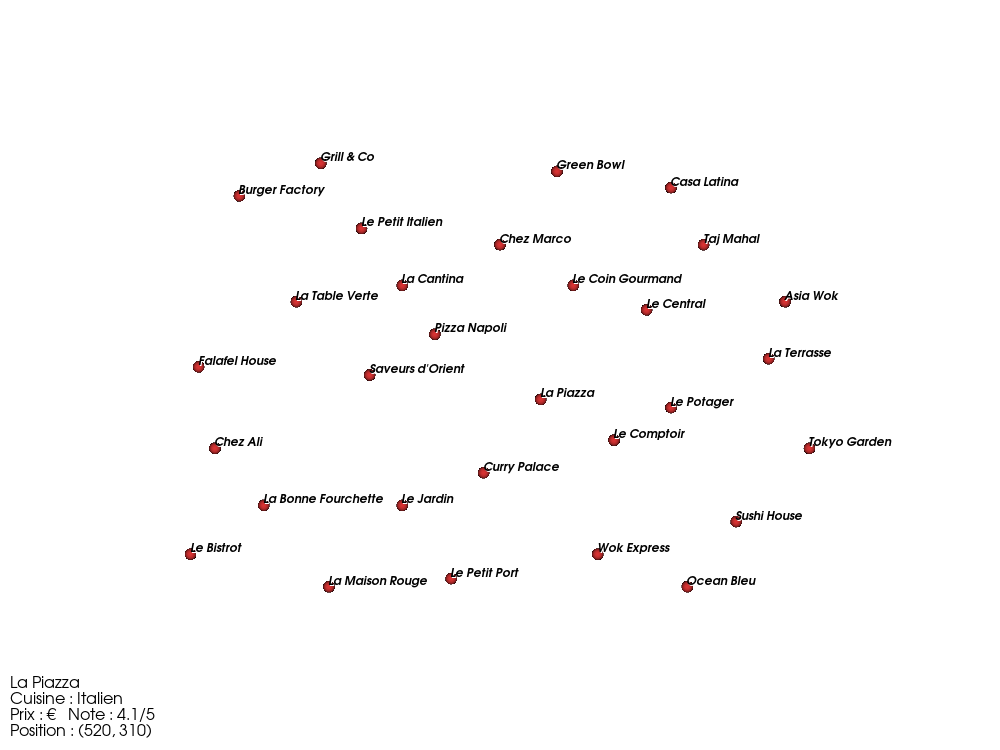
\includegraphics[width=0.85\textwidth]{partie1.png}
  \caption{Carte des restaurants, après un clic sur \emph{La Piazza}.}
  \label{fig:partie1}
\end{figure}

Deux tests (\texttt{pytest}) vérifient que les 30 restaurants sont bien lus
et que le point $i$ a bien les coordonnées du restaurant $i$.

% ====================================================================
\section{Partie 2 -- Diagramme de Voronoï}
% ====================================================================

% À compléter

% ====================================================================
\section{Partie 3 -- Recherche à partir d'une position}
% ====================================================================

% À compléter

% ====================================================================
\section{Partie 4 -- Restaurants voisins}
% ====================================================================

% À compléter

% ====================================================================
\section{Partie 5 -- Alternatives}
% ====================================================================

% À compléter

% ====================================================================
\section{Utilisation de l'IA}
% ====================================================================

\subsection*{Outil et tâches}

J'ai utilisé Claude Code (Anthropic) dans VS Code pour :
\begin{itemize}
  \item mettre en place la structure du projet ;
  \item écrire le code de la partie 1 et ses tests ;
  \item préparer une première version de ce rapport.
\end{itemize}

\subsection*{Exemple : une première version trop complexe}

La première version proposée pour la partie 1 faisait plus de 400 lignes :
vérification détaillée du fichier CSV (identifiants en double, positions
identiques\dots), options en ligne de commande, panneau latéral avec
légende, couleurs par type de cuisine. Elle fonctionnait, mais je n'arrivais
pas à la suivre dans son ensemble, et la plupart de ces ajouts n'étaient pas
demandés.

Je lui ai donc demandé une version plus simple. Elle est passée à environ
150 lignes en gardant l'essentiel : lecture, affichage, association
point--restaurant et clic. C'est cette version que j'ai conservée, et je peux
l'expliquer en entier.

\subsection*{Vérification et corrections}

Le code n'a pas toujours fonctionné du premier coup. Par exemple, l'IA avait
utilisé la méthode \texttt{AddActor2D}, qui n'existe pas dans la version de
VTK installée. L'erreur est apparue au lancement, et la méthode a été
remplacée par \texttt{AddActor}.

J'ai vérifié le reste en lançant les tests, en cliquant sur plusieurs
restaurants et en comparant les informations affichées avec le fichier CSV.

% ====================================================================
\section{Conclusion}
% ====================================================================

% À compléter

\end{document}
